\newpage
\section{Справочные сведения о походе}
\subsection{Общие справочные сведения о маршруте}
\begin{tabular}{ l l }
    Вид туризма: & пеший\\
    Категория сложности: & 1\\
    Место проведения: & Россия, Мурманская область, район Хибины\\
    Время проведения: & 5-12 августа 2022 г.\\
    Продолжительность похода: & 8 ходовых дней\\
    Протяжённость маршрута: & 117.7 км\\
\end{tabular}

\subsection{Подробная нитка маршрута}
ст. Имандра - р. Гольцовка - руч. Меридиональный - пер. Юмъекорр (н/к)- руч. Юмъекорруай -
ущ. Аку-Аку (рад.) - ущ. Звездочка - руч. Медвежий Лог - пер. Медвежий Лог (н/к) - руч. Чильмана -
р. Малая Белая - пер. Петрелиуса Западный (н/к) - руч. Петрелиуса - р. Кунийок - оз. Гольцовое -
руч. Партомйок - пер. Умбозерский (н/к) - р. Северный Каскаснюнйок - р. Каскаснюнйок - верш. Рыпнецк -
оз. Академическое - пер. Исток (1А, траверс) - р. Вудьяврйок - оз. Малый Вудъявр.

\subsection{График движения}
\begin{longtable}{|l|l|p{6cm}|p{6cm}|l|}
    \hline
    День & Дата & График заявленный & График реализованный & км\\
    \hline
    1 &
    05.08 &
    ст. Имандра - р. Гольцовка - руч. Меридиональный - пер. Юмъекорр (н/к) - руч. Юмъекорруай &
    ст. Имандра - р. Гольцовка - руч. Меридиональный - пер. Юмъекорр (н/к) - руч. Юмъекорруай &
    18.1
    \\
    \hline
    2 &
    06.08 &
    руч. Юмъекорруай - ущ. Аку-Аку (рад.) - ущ. Звездочка - руч. Медвежий Лог - пер. Медвежий Лог (н/к)
    - руч. Чильмана - р. Малая Белая &
    руч. Юмъекорруай - ущ. Аку-Аку (рад.) - ущ. Звездочка - руч. Медвежий Лог &
    14.1
    \\
    \hline
    3 &
    07.08 &
    р. Малая Белая - оз. "Хэмингуэя" &
    руч. Медвежий Лог - пер. Медвежий Лог (н/к) - руч. Чильмана - р. Малая Белая &
    9.7
    \\
    \hline
    4 &
    08.08 &
    оз. “Хэмингуэя” - пер. Петрелиуса Западный (н/к) - руч. Петрелиуса - р. Кунийок - оз. Гольцовое &
    р. Малая Белая - пер. Петрелиуса Западный (н/к) - руч. Петрелиуса &
    15.8
    \\
    \hline
    5 &
    09.08 &
    оз. Гольцовое - руч. Партомйок &
    руч. Петрелиуса - р. Кунийок - оз. Гольцовое  - руч. Партомйок - пер. Умбозерский (н/к) - р. Северный Каскаснюнйок &
	18.3
    \\
    \hline
    6 &
    10.08 &
    руч. Партомйок - пер. Умбозерский (н/к) - р. Северный Каскаснюнйок - переправа р. Каскаснюнйок &
    р. Северный Каскаснюнйок - р. Каскаснюнйок - переправа р. Каскаснюнйок &
	13.2
    \\
    \hline
    7 &
    11.08 &
    переправа р. Каскаснюнйок - верш. Рыпнецк - оз. Академическое &
    переправа р. Каскаснюнйок - верш. Рыпнецк - оз. Академическое &
	14.8
    \\
    \hline
    8 &
    12.08 &
    оз. Академическое - пер. Исток (1А, траверс) - р. Вудьяврйок - оз. Малый Вудъявр &
    оз. Академическое - пер. Исток (1А, траверс) - р. Вудьяврйок - оз. Малый Вудъявр &
	13.9
    \\
    \hline
    \multicolumn{4}{|l|}{Всего:} &
	117.7
    \\
    \multicolumn{4}{|l|}{Из них в зачёт:} &
    115.2
    \\
    \hline
\end{longtable}

Причины изменения заявленного графика:\\
\break
\textit{1. Основная причина}\\
Изначальная несбалансированность маршрута. Первоначально на день 2 планировалось три перевала с небольшими переходами.
День 3 был разгружен и планировался в виде небольшого линейного перехода.
В ходе обсуждения в МКК два перевала были убраны, на день 2 был назначен длинный переход и затем пер. Медвежий Лог.
Ненагруженный день 3 был оставлен без изменения. В итоге пройти пер. Медвежий Лог в день 2 просто не успели.
Случилась "естественная" балансировка маршрута.
В день 5, на который была запланирована полуднёвка на руч. Партомйок, после того как нагнали график,
решили пройти до более интересной стоянки.

\textit{2. Вторичная причина}\\
Задержка на пер. Медвежий Лог из-за непогоды на полтора часа (ещё полтора часа на перевале учтены в качестве времени на обед,
на который бы всё равно пришлось останавливаться).
Повлияла на то, что в день 3 не нагнали график.

\textit{3. Вторичная причина}\\
Долгие обеды). С одной стороны, обеды, конечно, можно было бы сократить на часть послеобеденного отдыха,
с другой - любование окрестными видами безусловно являлось неотъемлемой частью похода.
И как велосипедная поездка не может полностью заменить пешеходной прогулки, так и неподвижное раздумчивое созерцание гор
дополняет ощущения от видов "с хода".
Вероятно, в сумме причины 2 и 3 повлияли на то, что мы упустили где-то 2 часа и заночевали в день 4 не
на оз. Гольцовое, а на руч. Петрелиуса.

\textit{4. Выводы}\\
В результате от получившейся "естественной" балансировки поход только выиграл. Часть нагрузки с дней 2, 4, 6
распределилась на дни 3 и 5 и стала более равномерной. Вместо стоянки в районе оз. Гольцового,
которая была бы многолюдной и шумной (из-за транспортной доступности и соответственно большого количества туристов),
случилась стоянка на руч. Петрелиуса, где мы были одни. А вместо полуднёвки на проходном, и даже проезжем, руч. Партомйок,
получилась одинокая ночёвка на озерце после пер. Умбозёрский. Безопасность также не пострадала.
Напротив, пер. Медвежий Лог был пройден с утра со свежими силами. Пер. Умбозёрский же в силу его простоты и автодоступности
можно проходить в любое время дня.

\subsection{Расчет категории сложности пройденного маршрута}
Расчёт выполнен согласно "Методике категорирования пешеходного маршрута",
утверждённой решением Президиума ФСТП от 30 ноября 2016 года.

\textit{Для пешеходного маршрута 1 к.с.}

Продолжительность маршрута, $T$ = $8$ дней.\\
Протяжённость маршрута, $L_{\textsl{мар}}$ = $115$ км.\\

\centerline{Баллы за локальные препятствия $\textsl{ЛП}_{\textsl{б}}$}
Переправы ($1$ н/к ч/з р. Каскаснюнйок) - $0.5$ балла;\\
Перевалы ($4$ н/к пер. Юмъекорр, Медвежий Лог, Петрелиуса Западный, Умбозёрский) - $4$ балла;\\
Каньоны ($2$ н/к Аку-Аку, Звёздочка) - $2$ балла\\
$\textsl{ЛП}_{\textsl{б}}$ = $0.5 + 4 + 2$ = $6.5$ балла\\

\centerline{Баллы за протяжённые препятствия $\textsl{ПП}_{\textsl{б}}$}
Коэффициент труднопроходимости, $\textsl{К}_{\textsl{т}}$ = $0.40$\\
$\textsl{ПП}_{\textsl{ор}}$ = $12$ баллов\\
$L$ = $100$ км\\
$\textsl{ПП}_{\textsl{б}}$ = $\textsl{К}_{\textsl{т}} \times \textsl{ПП}_{\textsl{ор}} \times (L_{\textsl{мар}} / L)$
= $0.40 \times 12 \times (115 / 100)$ = $5.52$ балла\\

\centerline{Интегральная оценка категорируемого маршрута за район в баллах $\textsl{Р}_{\textsl{б}}$}
Географический показатель района, $\textsl{Г}$ = $9$ баллов\\
Суммарный перепад высот, $\Delta H$ = $9$ км\\
Коэффициент перепада высот, $\textsl{К}$ =  $1 + \Delta H / 12$ = $1 + 9 / 12$ = $1.75$\\
Показатель автономности маршрута, $\textsl{А}$ = $1$\\
$\textsl{Р}_{\textsl{б}}$ = $\textsl{Г} \times \textsl{К} \times \textsl{А}$ = $9 \times 1.75 \times 1$ = $15.75$ балла

\textbf{Общее количество баллов:} $\textsl{КС}_{\textsl{б}}$ =
$\textsl{ЛП}_{\textsl{б}} + \textsl{ПП}_{\textsl{б}} + \textsl{Р}_{\textsl{б}}$ = $6.5 + 5.52 + 15.75$ = $27.77$\\
\textbf{Требуемое количество баллов для маршрута $1$ к.с.:} $7$ - $20$

\textit{Для пешеходного маршрута 2 к.с.}

Продолжительность маршрута, $T$ = $8$ дней.\\
Протяжённость маршрута, $L_{\textsl{мар}}$ = $115$ км ($95.83\%$ от требуемой).\\

\centerline{Баллы за локальные препятствия $\textsl{ЛП}_{\textsl{б}}$}
Переправы ($1$ н/к ч/з р. Каскаснюнйок) - $0.5$ балла;\\
Перевалы ($4$ н/к пер. Юмъекорр, Медвежий Лог, Петрелиуса Западный, Умбозёрский) - $4$ балла;\\
Каньоны ($2$ н/к Аку-Аку, Звёздочка) - $2$ балла\\
$\textsl{ЛП}_{\textsl{б}}$ = $0.5 + 4 + 2$ = $6.5$ балла\\

\centerline{Баллы за протяжённые препятствия $\textsl{ПП}_{\textsl{б}}$}
Коэффициент труднопроходимости, $\textsl{К}_{\textsl{т}}$ = $0.40$\\
$\textsl{ПП}_{\textsl{ор}}$ = $24$ балла\\
$L$ = $120$ км\\
$\textsl{ПП}_{\textsl{б}}$ = $\textsl{К}_{\textsl{т}} \times \textsl{ПП}_{\textsl{ор}} \times (L_{\textsl{мар}} / L)$
= $0.40 \times 24 \times (115 / 120)$ = $9.2$ балла\\

\centerline{Интегральная оценка категорируемого маршрута за район в баллах $\textsl{Р}_{\textsl{б}}$}
Географический показатель района, $\textsl{Г}$ = $9$ баллов\\
Суммарный перепад высот, $\Delta H$ = $9$ км\\
Коэффициент перепада высот, $\textsl{К}$ =  $1 + \Delta H / 12$ = $1 + 9 / 12$ = $1.75$\\
Показатель автономности маршрута, $\textsl{А}$ = $1$\\
$\textsl{Р}_{\textsl{б}}$ = $\textsl{Г} \times \textsl{К} \times \textsl{А}$ = $9 \times 1.75 \times 1$ = $15.75$ балла

\textbf{Общее количество баллов:} $\textsl{КС}_{\textsl{б}}$ =
$\textsl{ЛП}_{\textsl{б}} + \textsl{ПП}_{\textsl{б}} + \textsl{Р}_{\textsl{б}}$ = $6.5 + 9.2 + 15.75$ = $31.45$\\
\textbf{Требуемое количество баллов для маршрута $2$ к.с.:} $21$ - $59$

Единственный маршрут из "Перечня классифицированных и эталонных туристских спортивных маршрутов и препятствий" от $2008$ года,
состоящий только из некатегорийных перевалов, содержит $5$ перевалов.
Кроме того наш маршрут не дотягивает $5$ км до требуемых $120$ км для маршрута $2$ к.с.
В связи с чем, полагаем возможным зачесть маршрут в качестве пешеходного маршрута $1$ к.с.

\subsection{Сведения о районе проведения похода}
Хибинский горный массив расположен на крайнем северо-западе материковой России, на Кольском полуострове.
Как и практически весь Кольский полуостров, находится за полярным кругом.
Представляет собой область радиусом примерно 20 км и площадью 1300 км$^{2}$.
Относится к среднегорью, высшая точка - вершина Юдычвумчорр (1200 метров над уровнем моря).

В силу своей транспортной доступности, район любим туристами, изучен и исхожен.
Поэтому повторять общеизвестные факты, изложенные в десятках туристких отчётах не будем.
Отметим лишь факты, непосредственно нас затронувшие.

Полярный день в этих местах заканчивается в июле. В течение августа долгота дня снижается с
19:30 до 15:15 часов (примерно). Средняя температура августа +14$\tccentigrade$ днём и +8$\tccentigrade$ ночью.
Возможны ночные заморозки. Вместе с сентябрём август на втором месте по количеству осадков после июля.

Хибинские перевалы в целом невысокой сложности, не более 2А. Общее число перевалов 90 (согласно каталогу
перевалов т/к Вестра). Все перевалы делятся по происхождению на две большие группы: ледниковые и тектонические.
Первые образовались при движении ледников и имеют форму широких седловин с пологими склонами.
Вторые - разломы и трещины - благодаря тектонической активности;
имеют отвесные стены и, обычно, разделены на несколько камер.

В августе и сентябре для знающего туриста ценность представляют съедобные ягоды и грибы, которые растут здесь в изобилии.
Сбор их, однако, замедляет перемещение.

\subsection{Состав спортивной группы}
\begin{tabular}{|l|l|l|l|}
    \hline
    ФИО & Год рождения & Должность в похоже & Туристский опыт\\
    \hline
    Гусев Роман Борисович &
    1981 &
    Руководитель, завхоз &
	3ГУ Алтай
    \\
    \hline
    Фомин Сергей Анатольевич &
    1981 &
    Штурман, летописец &
	1ГУ Алтай, 1ВУ
    \\
    \hline
\end{tabular}

\begin{figure}[H]
    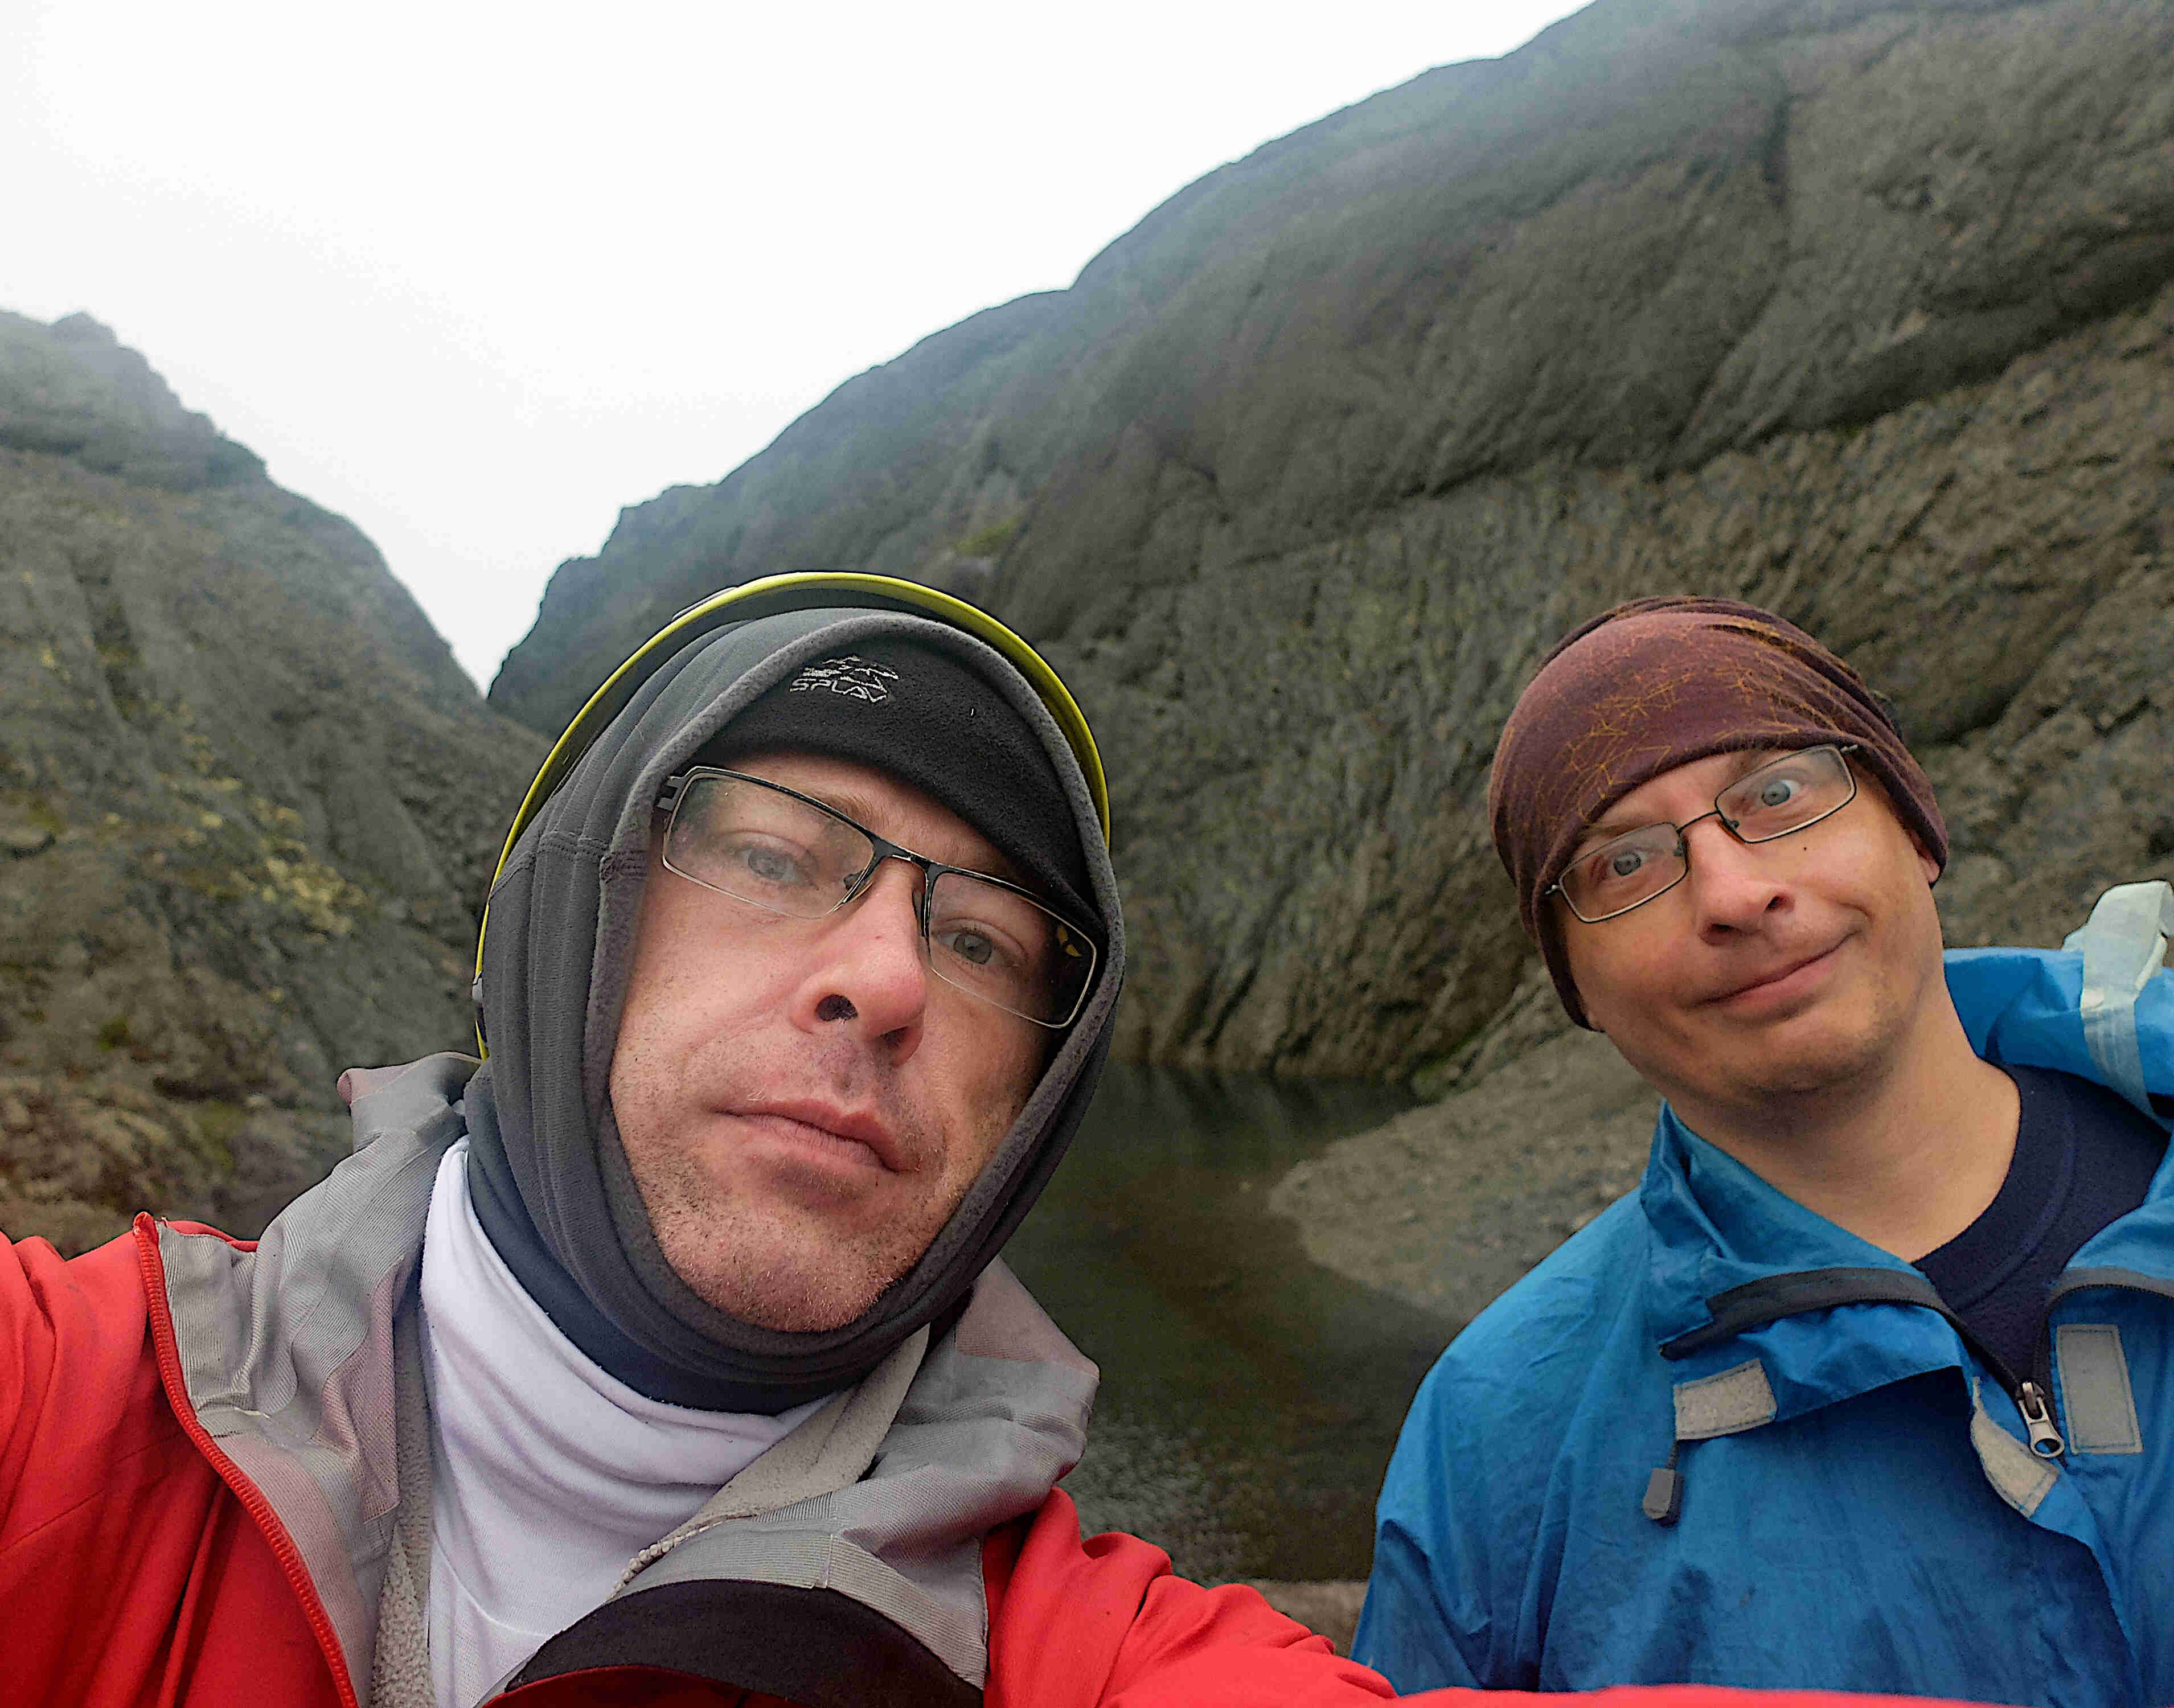
\includegraphics[width=16cm]{foto/Лица/mordas3.JPG}
    \caption*{Участники на пер. Юмъекорр, слева - Фомин С.А., справа - Гусев Р.Б.}
\end{figure}

\subsection{Обзорная карта маршрута}
\begin{figure}[H]
    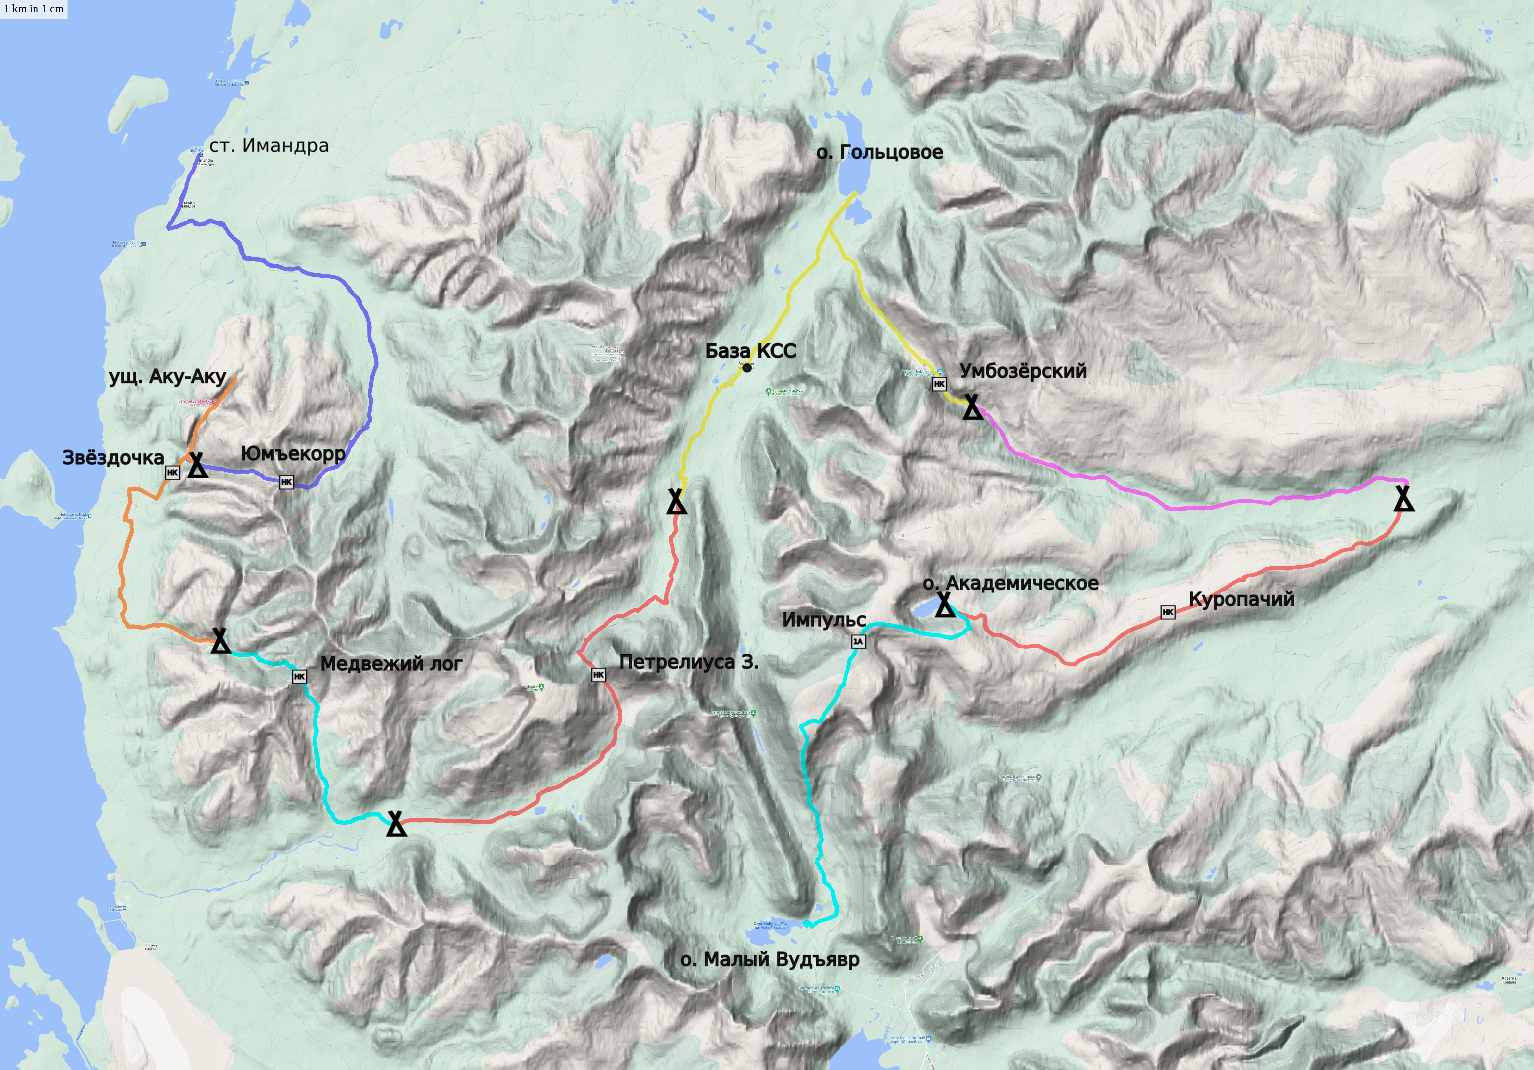
\includegraphics[width=18cm]{foto/overall_map.png}
\end{figure}


\subsection{Примечания по отчету}
Обозначения левый и правый относительного расположения в пространстве по умолчанию подразумеваются в орографическом смысле.

Километраж указан по GPS-треку, измеряется, за исключением отдельно обозначенного, по "горизонтали",
т.е. по проекции точек в пространстве на поверхность геоида. Точки трека записывались через интервал в 1, 2 и 3 минуты
(в разные дни); предполагаем, что ошибка gps-позиционирования, которая даёт прирост к к вычисленному расстоянию,
нивелируется cпрямлением полученного трека из-за большого по времени межточечного промежутка.
Отдельно при подсчёте расстояния в записанных треках удалены точки времени обеда и точки до старта и после финиша
(впрочем полтора часа обеда добавляют из-за ошибки GPS-позиционирования до 100 метров к вычисленному расстоянию),
точки привалов не удалялись, довесок для них составлял порядка +5 метров за привал.
В целом считаем округление расстояния до десятых километров соответствующим.

Набор и сброс высоты также указан по данным GPS-трекера.

У группы был с собой термометр, но поскольку наблюдения были несистемными, то отдельной таблицы температуры не приводится,
измеренные значения приводятся в тексте технического описания.

В тексте упоминается т.н. оз. "Хэмингуэя". Точное название найти не удалось.
Представляет собой пересыхающее озерцо, расположенное у расхождения троп на пер. Петрелиуса Западный и Восточный со
стороны долины р. Малой Белой. Координаты: N$67.7205^{\circ}$, E$33.5280^{\circ}$.

Сокращения в отчёте приняты общепринятые, единственно стоит подчеркнуть обозначения р. для рек и руч. для ручьёв.
